\section{Auslesen der Quests}
\subsection{Auslesen der Packages}

\begin{figure}[h] 
  \centering
     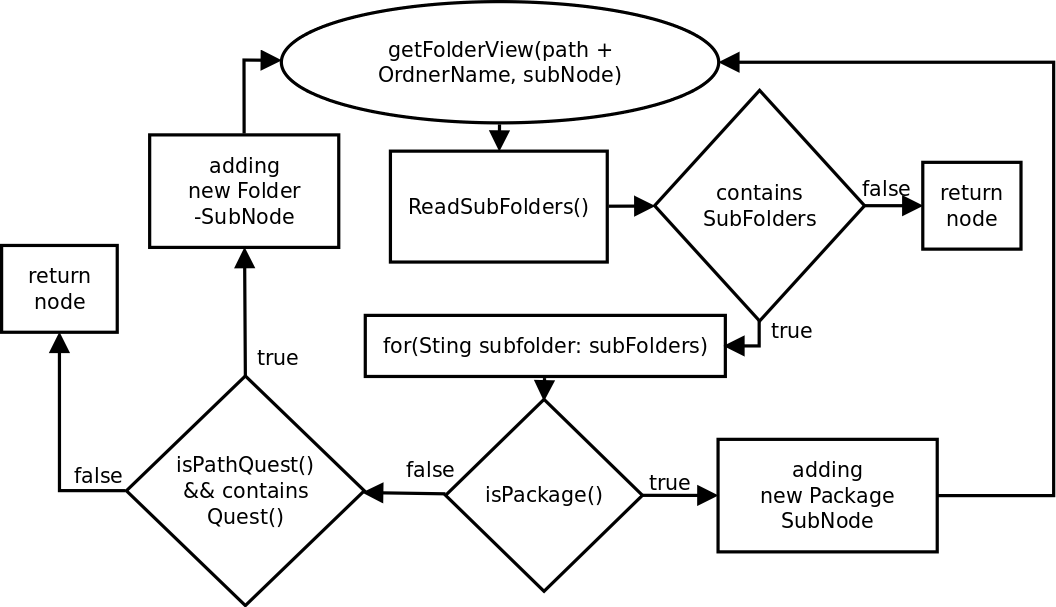
\includegraphics[width=1\textwidth]{./media/images/gui/package-tree-rekursion.png}
  \caption{Schematische Darstellung vom Auslesen der Packages}
  \label{fig:Package_Tree_Rekursion}
\end{figure}

Ob ein Ordner ein Package ist, wird mithilfe einer Rekursion ausgelesen. Der Ausgangspunkt dieser Rekursion bildet der Ordner \textbf{"`packages"'}. Dieser bildet auch den Hauptknoten. Nun wird \textit{\textbf{getFolderView()}} aufgerufen, und der relative Pfad und der Hauptknoten werden übergeben.

Von diesem Punkt aus wird in die nächsten Unterordner gewechselt. Dort wird nun zuerst überprüft, ob der gewählte Ordner Subordner enthält. Ist dies der Fall, wird durch die Liste der Unterordner mithilfe einer ForEach-Schleife durchiteriert.

Es wird nun überprüft, ob eines dieser Elemente ein Package ist. Trifft dies zu, wird das gerade iterierende Element als Unterknoten hinzugefügt und dieselbe Methode (\textit{\textbf{getFolderView()}}) wird nochmals aufgerufen.

Wenn das aktuelle Element kein Package ist, erfolgt erneut eine Überprüfung nach weiteren Quests im Unterordner. Werden solche gefunden, wird ein neuer Unterknoten erstellt und wiederum die eigene Methode aufgerufen.

Wenn diese Bedingung nicht zutrifft, wird der Hauptknoten wieder zurückgegeben.

\subsection{Überprüfungsiterationen und Rekursion}
\htlParagraph{isPackage()-Methode:}\\
Mithilfe von \textbf{isPackage()} wird eine Funktion aufgerufen, welche eine Iteration durchführt und alle Ordner mithilfe der \textit{\textbf{isPathQuest(path)}} Methode überprüft. Somit kann festgestellt werden, ob es sich bei dem geprüften Ordner um ein Package handelt.

\htlParagraph{isPathQuest()-Methode:}\\
Da eine Quest eine \textit{\textbf{ref.cmm}}, \textit{\textbf{description.html}} und eine \textit{\textbf{input.cmm}} haben muss, ist es möglich, anhand einer Iteration festzustellen, ob es sich bei diesen Ordnern um Quests handelt.

\htlParagraph{containsQuests()-Methode:}\\
Durch eine einfache Rekursion kann der gesamte Ordner mit seinen Unterordnern aufgeschlüsselt beziehungsweise auf Quests überprüft werden.

\begin{lstlisting}[language=JAVA]
	public static boolean containsQuests(String path){
		//Checking if there is a Quest in the Current Folder
		if(isPathQuest(path))
			return true;
		//Iterate through all other Folders
		else{
			List<String> subFolders = Quest.ReadFolderNames(path);
			if(subFolders != null){
				for(String subFolder : subFolders){
						return containsQuests(path + File.separator + subFolder);
				}
			}
		}
		return false;
	}
\end{lstlisting}



\begin{figure}[h] 
  \centering
     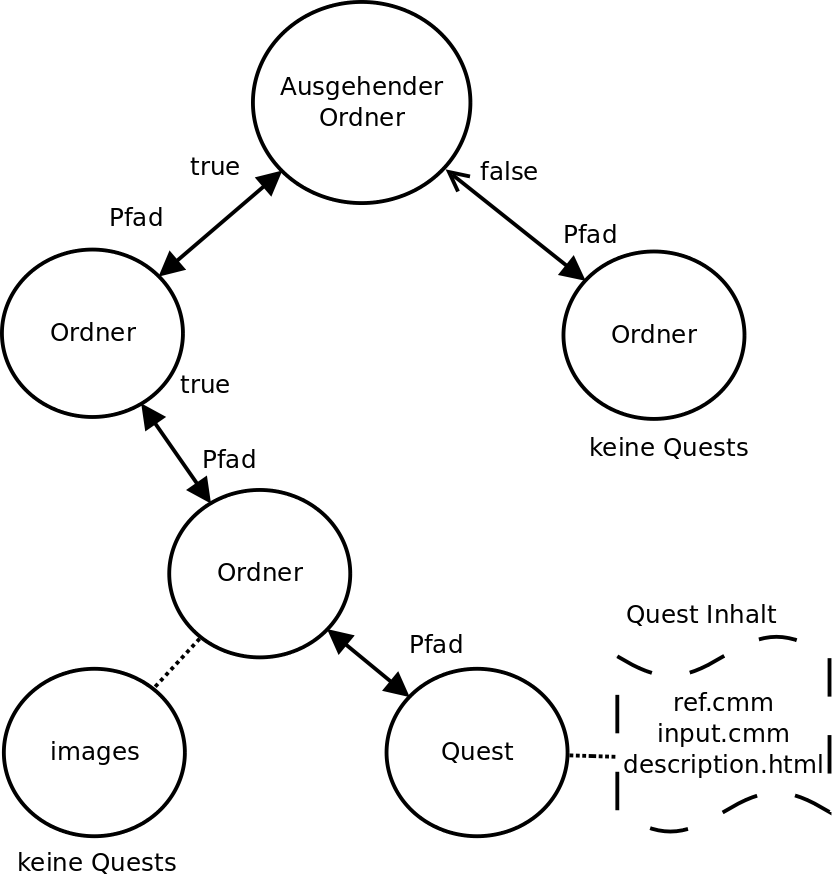
\includegraphics[width=0.5\textwidth]{./media/images/gui/quest-control-rekursion.png}
  \caption{Schematische Darstellung der Rekursion}
  \label{fig:JTree_Control_Rekursion}
\end{figure}

In der Abbildung \ref{fig:JTree_Control_Rekursion} wird ein beispielhafter Ordnerpfad aufgeschlüsselt. Der Ordner oberhalb des Questordners kann nun als Package erkannt werden.

\subsection{Auslesen einer Quest}
Damit eine Quest ausgelesen werden kann, ist es notwendig, dass alle benötigten Pfade verfügbar sind. Dazu zählen der Package-Pfad und der Ordnername der Quest.

Zuerst werden die Pfade, welche übergeben werden, gesetzt. Dann werden die enthaltenen Files auf Verfügbarkeit geprüft und der Status dementsprechend in den Variablen angepasst. Wenn die Dateien unvollständig sind oder der Pfad nicht verfügbar ist, wird die Quest als nicht funktionstüchtig erklärt.

Jetzt kann, wenn eine \textbf{quest.xml} vorhanden ist, diese ausgelesen werden. 

%Wenn Variablen keinen Wert zugewiesen bekommen haben, bekommen diese nun einen vordefinierten zugewiesen:
%\begin{itemize}
%	\item Der Titel wird auf den Ordnernamen gesetzt.
%	\item Der Status wird auf selectable gesetzt.
%	\item Das Attribut wird auf \textit{exercise} gesetzt.
%\end{itemize}

\subsection{Auslesen für die Quest-Ansicht}
Zuerst wird das Package mit der Methode \textbf{ReadPackage()} ausgelesen. Nun werden alle Quests, welche im Profil und im Package gespeichert sind, abgerufen. Damit die Quests des Packages mit den Questinformationen des Profils zusammenpassen, muss man diese mit Schleifen zusammenfügen. Dies geschieht, indem man die Pfade der im Profil gespeicherten Quests mit den vom Package ausgelesenen Quests vergleicht. Somit wird der Status, das Datum und die zuletzt verwendete Datei der Quest abgeglichen.

\htlParagraph{Abgleichen der gesperrten Quests:}\\
Um Quests, welche erst freigeschaltet werden, wenn andere erledigt wurden, freischalten zu können, ist wiederum ein Abgleich nötig. Dieser wird mit einer For-Schleife erledigt. 

Hierbei wird der Ordnername mit der Variable \textbf{previousFolder} abgeglichen. Hier musste besonders darauf geachtet werden, dass nur Quests geändert werden, bei denen der Status auf \textbf{locked} steht.

